%--------------------------------------------------------------------------------------------------%
%   Template infos:
%   Version:    1.0
%   Last Mod:   20170307    
%         By:   Juan Medina juancamilomedina1989@gmail.com
%   Author:     Juan Medina juancamilomedina1989@gmail.com
%--------------------------------------------------------------------------------------------------%
%   Thesis infos:
%   Author: William Piron
%   Tutor: François Delbot
%-------------------------------------------- PREAMBLE --------------------------------------------%
\documentclass[12pt,twoside]{report}
\usepackage[a4paper,width=150mm,headheight=110pt,top=25mm,bottom=25mm]{geometry}
\usepackage[utf8]{inputenc}
\usepackage{listings}
\usepackage{graphicx}
\usepackage{pgffor} 
\usepackage{float}
\usepackage{graphics} 
\usepackage{fancyhdr}
\usepackage[final]{pdfpages}

\graphicspath{{Images/}}

\usepackage[round, numbers,authoryear]{natbib}
\usepackage{color}
\usepackage[dvipsnames]{xcolor}

\definecolor{mycolor}{RGB}{30,75,180}
\definecolor{mycolor2}{RGB}{40,75,90}
% Lund colors
\definecolor{LUGreen}{RGB}{173,202,184}
\definecolor{LUPink}{RGB}{233,196,199}
\definecolor{LUBlue}{RGB}{0,0,128}
\definecolor{LUBronze}{RGB}{156,97,20}
\definecolor{LUblue}{RGB}{185,211,220}
\definecolor{LUGrey}{RGB}{77,76,68}

\usepackage[colorlinks = true,
            linkcolor = mycolor,
            urlcolor  = mycolor,
            citecolor = mycolor,
            anchorcolor = mycolor]{hyperref}

\usepackage[hypcap=true,font={small,it}]{caption}
\usepackage{indentfirst}
\usepackage{caption}
\usepackage{shorttoc}

%paragraph indentation
\setlength{\parindent}{4em} 
%Line spacing
\renewcommand{\baselinestretch}{1.3}

\captionsetup{belowskip=2pt,aboveskip=2pt}
%\bibliographystyle{abbrvnat}
\bibliographystyle{plain}

\renewcommand{\chaptername}{}

\renewcommand{\figureautorefname}{figure} % lower case default ref
\renewcommand{\tableautorefname}{table} % lower case default ref
\newcommand{\latex}{\LaTeX\xspace}
\newcommand{\mcite}[1]{\textcolor{mycolor}{\citeauthor{#1} (\citeyear{#1})}}
\newcommand{\hcite}[1]{(\textcolor{mycolor}{\citeauthor{#1}, \citeyear{#1}})}
\newcommand{\source}[1]{\caption*{Source: {#1}} }

\renewcommand{\listfigurename}{Liste des figures}
 
\renewcommand{\listtablename}{Liste des tableaux}

%----------------------------------------------------------------------------------------------------%

%--------------------------------------------- DOCUMENT ---------------------------------------------%
\begin{document}
%\fancyhead[RO,LE]{}

% Title page
    \begin{titlepage}
\begin{center}

\includegraphics[width=0.7\linewidth]{Images/Logo_Universite_Paris-Nanterre.png}
\end{center}
\vspace{2cm}
    \begin{center}
        \vspace*{1cm}
        
        {\LARGE \textbf{Gamification de l'enseignement en Recherche Opérationnelle}}
        
        \vspace{0.5cm}
        %SOUS TITRE
        
        \vspace{1.5cm}
        par \\
        \vspace{1.5cm}
       William Piron - william.piron77@gmail.com \\
       Étudiant en 2ème année de Master MIAGE \\
       Université Paris-Nanterre
                
        \vspace{1.0cm}
    \end{center}

\vfill
\textcolor[rgb]{0.5,0.5,0.5}{
    \begin{flushleft}
    { \small
    Mémoire de Master MIAGE \\
    Année 2018-2019 \\
    Tuteur enseignant : François Delbot \\
    }
    \end{flushleft}
}
      
\end{titlepage}


    

% Table of contents, list of figures, and list of tables
    {\hypersetup{linkcolor=black}
        %\tableofcontents
        \shorttoc{Sommaire}{1}
        \listoffigures
        \listoftables
    }
        {\hypersetup{linkcolor=mycolor}}
        
    
    \cleardoublepage
% Acknowledgements
    \chapter*{Remerciements}
    Ce travail de recherche et de rédaction n'aurait pas été possible sans l'aide et le soutien de plusieurs personnes. \par

Tout d'abord, je tiens à remercier chaleureusement M. François Delbot, Maître de Conférences à l'Université Paris-Nanterre pour son soutien et son accompagnement tout au long de mon parcours au sein de la MIAGE de Nanterre. Son suivi, ses encouragements, ses conseils et ses retours ont été essentiels tout au long de mon cursus et plus encore lors de la réalisation de ce mémoire de fin d'études. \par

Je tiens également à remercier M. Philippe Roulet, Responsable de l'Équipe Centrale Data chez Placoplâtre Saint-Gobain, mon tuteur en entreprise lors de mon stage de fin d'études, pour sa disponibilité, ses conseils et son encadrement durant ce stage et mes précédents passage au sein de son équipe lors de mon cursus MIAGE. \par

Enfin, je tiens à remercier l'ensemble des enseignants et professeurs du département MIAGE de l'Université Paris-Nanterre, ainsi que mes proches pour les conseils et importantes leçons qu'ils m'ont prodigués tout au long de mon parcours.
        
    \cleardoublepage
% Introduction
    \chapter{Introduction} 
    Ce mémoire s'inscrit en conclusion d'un cycle d'études en Licence puis Master MIAGE au sein de l'Université Paris-Nanterre. Au delà de s'additionner aux diverses évaluations dans la validation des acquis, il a pour but de développer l'esprit de recherche et de synthèse des étudiants au sein d'une démarche de questionnement et d'analyse.\par
Ce document encadré par M. François Delbot, maître de conférences à l'Université Paris-Nanterre, est le fruit de cette démarche.

\section{Motivations}
Années après années, l'enseignement est confronté à un problème récurrent : capter l'attention des élèves et étudiants afin de leur transmettre de la meilleure manière possible des connaissances. Selon le domaine étudié, la composition des groupes d'apprenants et leurs personnalités propres, la méthode à appliquer et les moyens utilisés sont variés, tous comme leurs résultats. \par
Tous les étudiants n'attendent pas la même chose d'un enseignement et ne s'y investissent pas avec la même intensité. Certains doivent être motivés ne serait ce que pour assister aux enseignements quand d'autres ont besoin d'un encadrement ou d'une réalisation concrète et précise. \par
La question d'une méthode d'enseignement permettant de répondre ce besoin de manière globale, adaptée à toutes les catégories d'apprenants et aisément mise en place par les enseignants se pose alors.

\section{Objectif du mémoire}
L'objectif de ce mémoire est de poser la question de la gamification appliquée à l'enseignement, plus particulièrement à celui de la Recherche Opérationnelle dans le cadre de la licence MIASHS parcours MIAGE de l'Université Paris-Nanterre. \par
Nous définirons la gamification et ses principes, le cadre dans lequel nous comptons l'évaluer et dans quels objectifs, avant de d'analyser les résultats de ses applications dans d'autres enseignements et domaines par d'autres équipes et chercheurs. \par
Nous proposerons ensuite une expérience pouvant être réalisée au sein de l'Université afin de comparer l'enseignement concerné avec mise en place de gamification par rapport à l'enseignement dit traditionnel de la matière.
    
    
    \cleardoublepage
% Definitions
    \chapter{Définition de la gamification}
    \section{Description et objectifs}
La gamification, ou ludification, est définie comme l’application d’élément issus de jeux, jeux vidéo ou autre activités ludiques à d’autre domaines. Ces éléments sont dans la majorité des cas la mise en place d’un système de score à points, d’un statut lié au niveau ou temps de jeu, de l’utilisation de tableaux de bord, de compétition (coopérative ou non) et de règles de jeu à suivre. La gamification est généralement appliquée dans le cadre du marketing afin d’augmenter l’engagement des potentiels clients envers un produit ou service.\par
Le terme et son application sont depuis quelques années devenu très à la mode dans d’autres domaines que le marketing, que ce soit lors de projets internes à une entreprise, de séminaires de cohésion d’équipe ou, dans le cadre de ce mémoire le cas qui nous intéresse, l’enseignement d’une discipline.

\section{Les mécaniques de la gamification}
Basé sur les travaux de Gabe Zihermann et d'Andrzej Marcsweski, Sarath Koppolu~\cite{gamif-thesis} définit les cinq principes de la gamification comme suit : 
\begin{enumerate}
    \item "Purpose" : la gamification doit avoir un but clair et défini dans le processus où elle est appliquée, processus dont les participants ont une connaissance suffisante pour comprendre et accepter son application
    \item "Progress" : l’accompagnement de la progression des participants, notamment via l’apprentissage de nouvelles compétences, leur affûtage ou les retours réguliers d’expérience par exemple
    \item "Proficiency" : travailler sur la motivation des participants à faire les choses parce qu’ils l’apprécient plutôt que pour simplement en obtenir quelque chose
    \item "Pride" : récompenser les participants pour leur apporter de l’estime d’eux-mêmes et maintenir leur intérêt
    \item "People" : construire le processus autour des gens au lieu de les considérer comme une simple entité du système gamifié. Construire autour des envies et besoins des gens plutôt que du système
\end{enumerate}\par

Basé sur le Framework Octalysis~\ref{fig:octalysis}, il est possible de définir et répartir divers comportements, processus et moteurs de gamification entre le "cerveau gauche" (accomplissement, possession, rareté) et le "cerveau droit" (responsabilisation, influence sociale, imprédictibilité). Il sépare également les bons comportements et influences de la gamification des néfastes, en "White hat" et "Black hat gamification". La seconde utilise la peur, l’incertitude, la perte d’opportunité pour maintenir les participants engagés, mais entraîne de nombreuses pertes pour ceux-ci à terme, que ce soit en quittant le système ou en développant des addictions diverses, là où la première encourage la créativité, récompense, encourage et aide les participants à s’améliorer afin de les maintenir engagés.

\begin{figure}
    \centering
    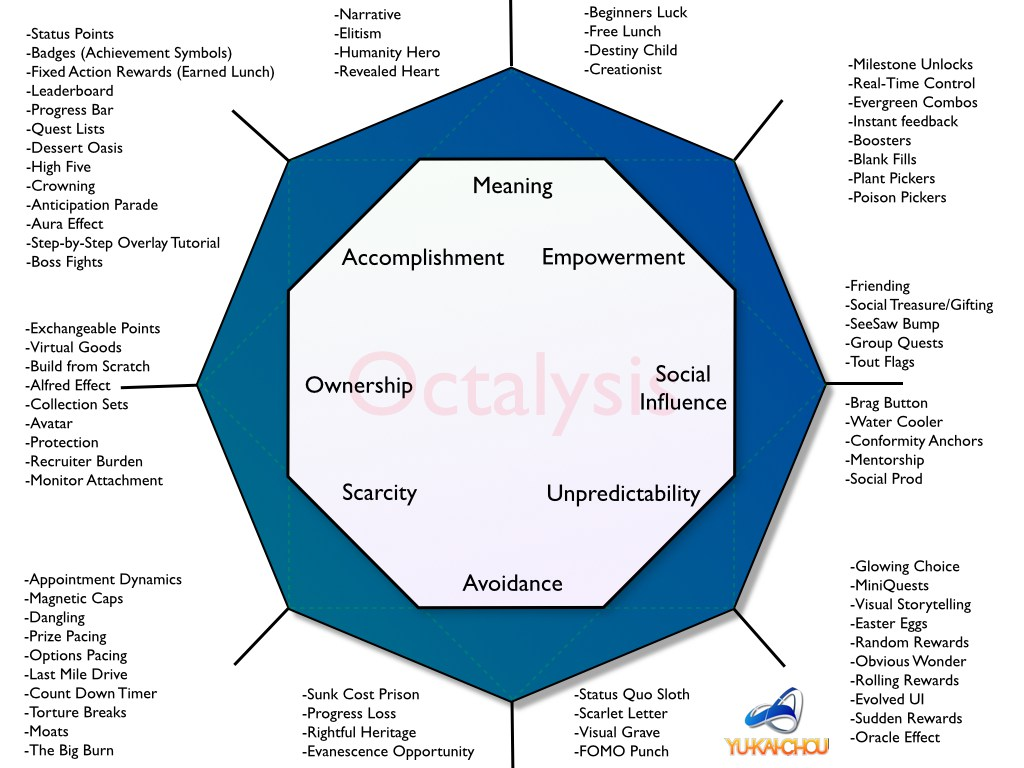
\includegraphics[width=0.9\linewidth]{Images/The-Octalysis-Framework.jpg}
    \caption{Framework Octalysis}
    \source{Yu Kai Chou, 2013}
    \label{fig:octalysis}
\end{figure}

\section{Types de participants}
En se basant sur la taxinomie de Richard Bartle et les travaux de Alexandra Iosup et Dick Epema~\cite{gamif-educ, gamif-taxonomy}, on peut identifier quatre types d'étudiants dans le cadre d'un enseignement gamifié~\ref{fig:bartle} :
\begin{itemize}
    \item Les "Explorers" sont ceux qui aiment comprendre et découvrir le monde, les curieux. Ils sont à la fois intéressés par la qualité et la quantité des enseignements
    \item Les "Achievers" sont ceux qui aiment réussir les challenges auxquels ils sont confrontés, les ambitieux qui en plus de valider le cursus le font avec les meilleurs résultats
    \item Les "Socialisers" sont ceux qui participent principalement parce que d’autres personnes comme eux le font également ; réussir le cursus les intéresse surtout s’ils maintiennent leur cercle social
    \item Les "Winners", ou "Killers" dans la taxinomie originale, sont ceux qui veulent réussir au dépend des autres participants. Pour eux, un challenge n’a de sens que s’il n’y a qu’un seul gagnant, si possible eux. Cette tendance à la compétitivité peut être autodestructrice, et mener à l’ennui, au burn-out, voire à la dépression
\end{itemize}

\begin{figure}
    \centering
    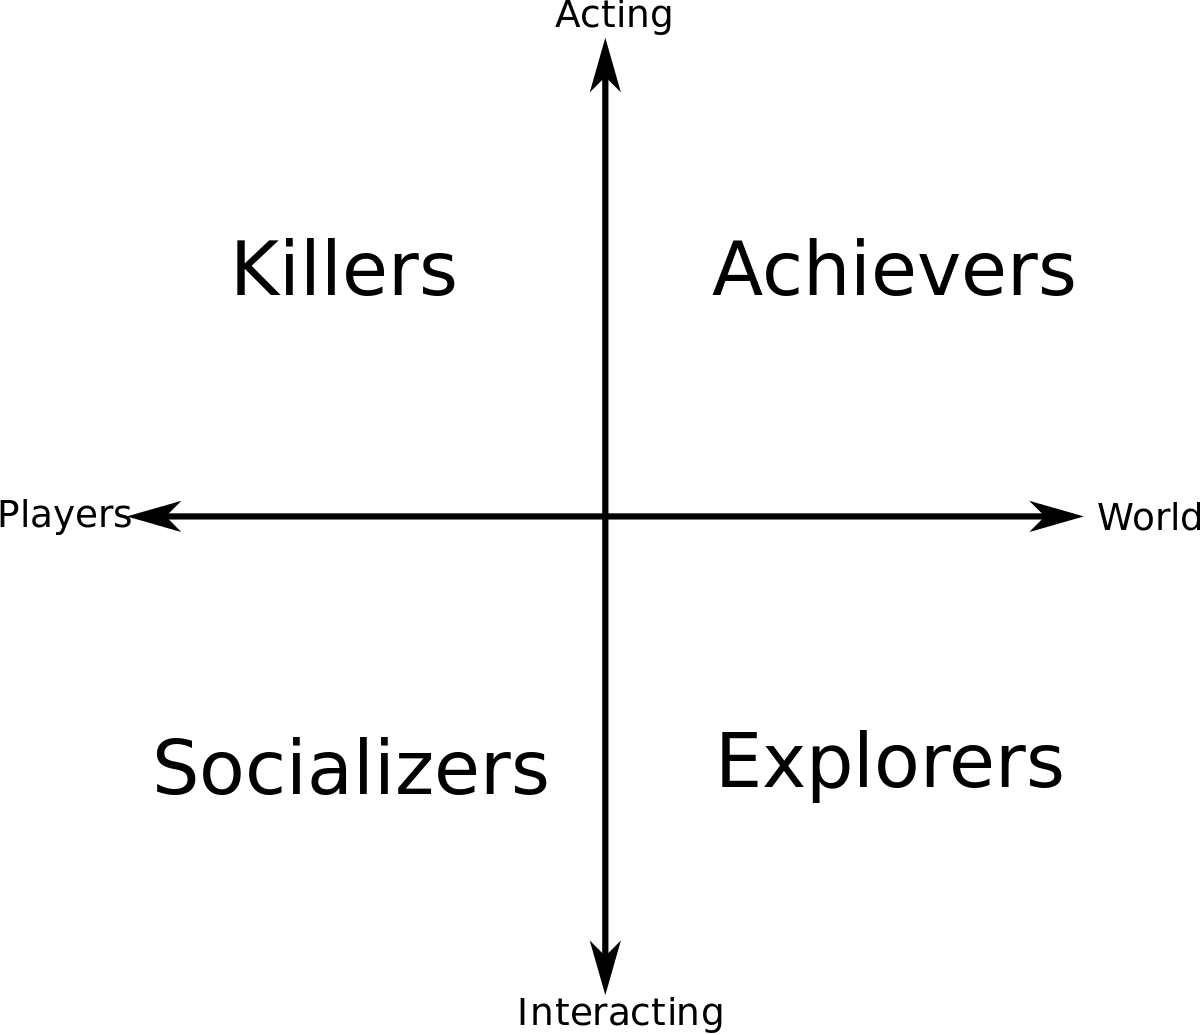
\includegraphics[width=0.5\linewidth]{Images/Character_theory_chart.png}
    \caption{Catégories de joueurs}
  
    \source{Richard Bartle, 1996}
    \label{fig:bartle}
\end{figure}


\section{Différence avec les "Jeux sérieux"}
Un jeu sérieux, de l'anglais "serious game", est une activité mêlant une intention pédagogique ou informative ("sérieuse") avec des ressorts ludique, ici le jeu. On peut résumer un jeu sérieux à un jeu de société, de rôle ou vidéo qui s'éloigne du seul but de divertissement ou amusement. \par
La vocation d'un jeu sérieux est de rendre sa composante sérieuse attrayante via son côté ludique et interactif. Là où la gamification vise à introduire à un enseignement ou projet des mécaniques et aspects issus de jeux pour en augmenter l'engagement et l'efficacité, les jeux sérieux sont d'avantage des outils complémentaires à l'enseignement. Ils permettent d'apprendre ou de consolider des connaissances via le jeu, là où la gamification est une forme d'apprentissage et de réalisation à part entière.
     
     \cleardoublepage
% State of the art
    \chapter{Etat de l'art}
    \section{La gamification comme motivation}
\subsection{Expérience de "sensing"}
La première amélioration attendue après gamification est l'amélioration de la motivation et de l'implication des participants. Dans le cadre d'une activité de "participatory sensing" réalisée via une application mobile~\cite{gamif-partici},  les participants vont relever diverses informations à des endroits qui leur sont indiqués, par exemple les conditions météorologiques et la fluidité du trafic routier à un croisement de rue donné. L'expérience réalisée ici récompensait par de petites sommes d'argent les participants pour chaque tâche effectuée, sommes augmentant selon la distance parcourue et la tâche effectuée. L'expérience consistait à rajouter un système de badges, de classement et de prix pour les tâches plus complexes afin de motiver davantage les utilisateurs sans augmenter les sommes à verser.\par

Les participants ont été répartis dans trois groupes, ou clusters, en plus d'un groupe témoin :
\begin{itemize}
    \item Le premier cluster sépare les utilisateurs par niveaux, augmentant selon l'expérience obtenue via les tâches réalisées
    \item Le deuxième utilise un système de score augmentant avec le nombre de tâches réalisées et leur complexité
    \item Le troisième distribue des badges au participants sans système de classement
    \item Enfin, le groupe témoin utilise le système de base de l'application, à savoir un système de points marqués en fonction des tâches, échangeable contre des sommes d'argent
\end{itemize} \par

Les tâches sont réalisés grâce à la géolocalisation des utilisateurs. Elles consistent à aller jusqu’à un endroit indiqué par l’application et à valider  le déplacement au point marqué sur la carte. Les points ou badges indiqués dans la définition de la tâche sont ensuite attribués. Le déplacement vers ces points d’intérêt permet de recueillir les données de l’environnement parcouru par les utilisateurs.

\subsection{Impact sur la participation}
Là où le groupe témoin présente une participation de 53\% au tâches proposées, avec motivation financière à la clé, la mise en place de la gamification la fait passer à 73\%. On remarque que la mise en place de niveau d'expérience, qui en plus de monter au fur et à mesure récompensent avec davantage de points lorsque plus élevé, entraîne une augmentation de la probabilité de participation~\ref{fig:rewards}. Bien que le gain en point soit plus faible au démarrage, la participation augmente globalement avec la montée de niveau, et par conséquent avec l'augmentation de la gratification. \par

Les dix-huit participants à cette expérimentation ont tous montré une meilleure implication dans la collecte d'informations. Quand questionnés sur la raison principale, selon eux, de cette participation, la majeure partie a répondu que le fait que tout le monde participait et qu'ils voulaient atteindre des niveaux plus élevés étaient les facteurs les plus motivant. \par

Les auteurs envisagent de réitérer une expérience similaire dans le futur afin d'observer l'impact plus précis des points marqués durant la participation, ainsi que la présence d'une limite dans le temps pour réaliser la tâche, ainsi qu'en utilisant un échantillon de participants plus grand.


\begin{figure}
    \centering
    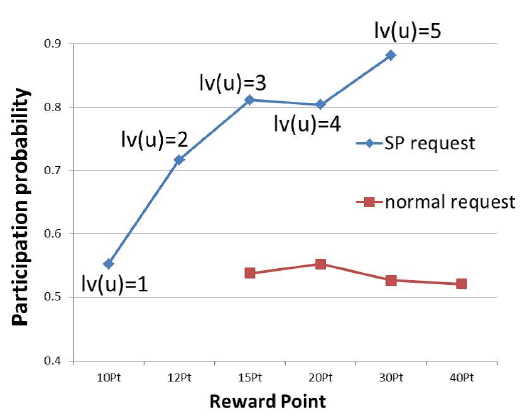
\includegraphics[width=0.7\linewidth]{Images/sensing-participation-figure.png}
    \caption{Probabilité de participation VS Points de récompense}
    \source{\cite{gamif-partici}}
    \label{fig:rewards}
\end{figure}

\section{La gamification dans l'enseignement}
\subsection{Définition du contexte}
Alexandru Iosup et Dick Epema~\cite{gamif-educ} se sont intéressés au problème de la baisse du nombre d'inscriptions dans les universités techniques aux Pays-Bas et en Europe, ainsi qu'à la baisse de la qualité de l'enseignement des sciences durant la dernière décennie\footnote{D'après les auteurs ; voir le rapport "Dijsselbloem Committee (2008) End report to Parliamentary
investigation (2007–2008), Dutch Government, Second
Chamber Report"}. Afin d'attirer des étudiants d'horizons variés et de maintenir leur intérêt et leur implication dans les enseignements, les auteurs ont mis en place des éléments de gamification sur deux cursus : un cours de première année en "Computer Organization", équivalent Licence, et un cours supérieur en "Cloud Computing", équivalent Master. \par

Les deux cursus choisis ont été retravaillés autour de la gamification et de manière à intégrer tous les types possibles de participants~\ref{fig:bartle}. Plusieurs chemins d'avancement sont proposés au sein des différents cours, suffisamment longs et complets pour proposer de nombreuses options. Par exemple, il est possible à un élève de choisir une option lui permettant de suggérer des points à aborder en cours. Dans chaque enseignement, les apprenants sont regroupés en équipes. Chaque cours se termine par une évaluation, analysée via des techniques de data mining pour déterminer les performances, intérêts et lacunes éventuelles de tous les participants afin d'adapter le cours suivant.

\subsection{Mécaniques et dynamiques de gamification}
Dans le contexte de l'enseignement de ces deux cursus, MM. Iosup et Epema ont mis en place sept outils afin d'encadrer le processus de gamification, les récompenses et le parcours des apprenants :
\begin{itemize}
    \item Trois mécaniques principales de jeu :
    \begin{enumerate}
        \item un système de points, basé sur les performances des participants, aussi bien aux évaluations que leur participation aux cours
        \item un classement anonyme afin d’encourager la compétition sans décourager les étudiants ou les pousser au surmenage
        \item un système conjoint de niveau/accès/pouvoir, qui correspondent respectivement à l’accumulation de points, à ce que peut voir et faire le participant dans le cadre de jeu, et aux actions réalisables par les participants dans le cadre du cursus ou du cours
    \end{enumerate}
    \item Quatre dynamiques d'encadrement du jeu :
    \begin{enumerate}
        \item un système de badges servant à montrer ses réussites et son niveau dans le cursus
        \item des tutoriels pour entrer dans le système de jeu et en comprendre rapidement le fonctionnement
        \item des boucles d’engagement pour maintenir l’intérêt des participants via une inclusion dans une équipe ou structure où chaque participant est essentiel à son fonctionnement
        \item du contenu optionnel à débloquer via la participation et l’avancement, afin d’impliquer et motiver les participants
    \end{enumerate}
\end{itemize}

\subsection{Impact sur l'enseignement}
De cette application de la gamification à ces deux enseignements ressort un passage de 65\% à 75\% de réussite des élèves y prenant part. Les auteurs corrèlent également l'augmentation de la satisfaction des étudiants à l'évolution ludique des cursus, grâce aux retours des étudiants et de l'expérience des enseignants concernés, tout en précisant qu'il ne s'agit pas nécessairement d'une relation de cause à effet. Une amélioration du taux de réussite des étudiants de première année a également été constatée et attribuée à la dynamique sociale entraînée par la gamification, où les interactions et compétitions motivent les étudiants à venir et s’impliquer. La multiplicité des chemins et contenus optionnel à débloquer fonctionne très bien en Master et doit être améliorée pour les premières années d’après les auteurs, afin d’intensifier leur participation. \par

L’étude fait ressortir les bénéfices de la gamification dans ces enseignements aussi bien pour les étudiants, qui apprennent mieux et s’impliquent plus, que pour les enseignants, dans leur relation avec les participants qui tend à s’améliorer et s’approfondir. Elle permet également à ces derniers de mieux percevoir leurs axes d’améliorations et leurs domaines de prédilection, y compris lors qu’ils les ignorent au début du cursus. Cependant, la mise en place efficace d’un enseignement gamifié peut être compliquée si le nombre d’étudiants en trop important, si les enseignants ne sont pas complètement à l’aise avec l’enseignement classique ou si le support de l’université ou de la faculté n’est pas présent.

\section{Les différentes applications de la gamification}
\subsection{Analyse documentaire}
Durant les dix dernières années, la question de la gamification a été de plus en plus abordée en France~\ref{fig:trends}, mais également dans le reste du monde. De nombreux articles et études ont été réalisées, afin d'analyser différents contextes, domaines et méthodes appliquées et leurs résultats. L'étude suivante~\cite{gamif-review} regroupe ainsi vingt-quatre articles et autres études provenant de bases de données variées comme par exemple Scopus, ACM Digital Library ou Google Scholar. \par

Les auteurs ont effectué leur recherche documentaire sur les articles évalués par les pairs de ces bases, puis l'ont ensuite raffinée avec les quatre critères suivants : les recherches sont empiriques (c’est-à-dire basée sur des données historiques), les méthodes sont clairement expliquées, les types de motivations mises en place durant l’étude sont explicitées, et celle-ci est réellement centrée sur la gamification plutôt que sur des jeux (du type jeux sérieux).\par

La question du fonctionnement réel et vérifié de la gamification est celle se dégageant et liant les articles ainsi obtenus, explicitement ou formulée différemment. Les principales données analysées sont majoritairement les résultats comportementaux des participants et dans une moindre mesure des comportements psychologiques. Selon les auteurs, une seule de ces études se base sur de vraies mesures psychométriques concrètes, sans que cela n'invalide les autres. \par

Les types de motivations relevés sont :
\begin{itemize}
    \item un système de points (scores ou simple accumulation)
    \item un classement des participants
    \item un système de badges ou de succès obtenus selon les réalisations
    \item des niveaux d'expérience pour marquer l'avancement
    \item une histoire ou un thème afin de mettre en place une dynamique de jeu de rôle
    \item des buts clairement définis à atteindre pour progresser
    \item des retours d'informations suite aux actions des participants et notamment de leurs progrès
    \item un challenge suffisant pour garder les participants dans le jeu
\end{itemize}

\begin{figure}
    \centering
    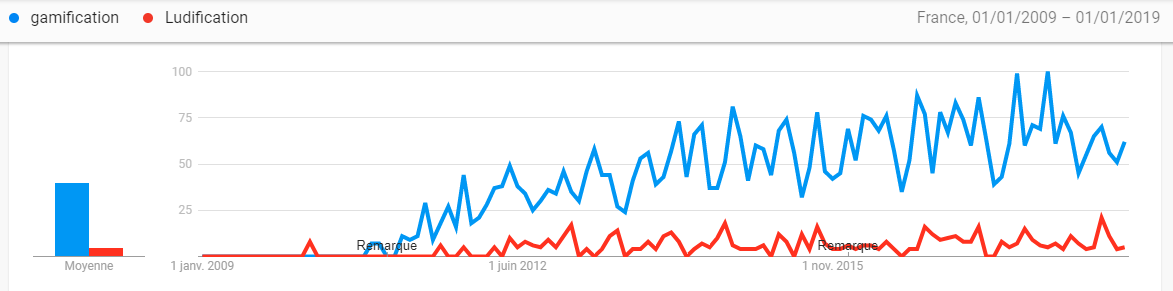
\includegraphics[width=\linewidth]{Images/trends_gamification.png}
    \caption{Évolution de l'intérêt pour la gamification/ludification sur le moteur de recherche Google}
    \source{\cite{gamif-trends}}
    \label{fig:trends}
\end{figure}

\subsection{Données relatives à l'enseignement}
Neuf des articles étudiés ici sont relatifs à l'éducation et à l'apprentissage en général. Comme la majorité des articles traités par Mme Koivisto et MM. Hamari et Sarsa~\cite{gamif-review}, ils font ressortir l’efficacité de la gamification dans le domaine où elle est mise en place. Il est cependant soulevé que l'efficacité finale est variable, bien que globalement positive, et dépend en grande partie de la motivation préexistante des participants pour l’activité proposée. Les mécaniques de jeu mises en place jouent également un rôle et peuvent influencer les résultats. \par 

Il ressort également que dans le domaine de l’enseignement, on constate une amélioration de la motivation, de l‘implication et de la satisfaction des apprenants. En contrepartie, il apparaît également une augmentation de la compétitivité, des risques de mauvaise évaluation de la difficulté d’une tâche et d’erreurs de conception. \par

L'étude pointe cependant que certaines différences de méthodologie et d'échantillonage dans les groupes étudiés peuvent limiter certaines conclusions des auteurs. Ils relèvent notamment certains groupes qu'ils estiment de petite taille ($N=20$ par exemple), sans groupe de contrôle ou sur des durées qui leur semblent courtes. Les résultats sont essentiellement issus des retours directs des participants et sont majoritairement liés à leur comportement durant ces expériences. Enfin, il aurait fallu pour eux que tous les types de motivations possibles soient évalués dans une même étude, ainsi que tous les résultats comportementaux et psychologiques.

    
    \cleardoublepage
% Experience
    \chapter{Expérience}
    \section{La Recherche Opérationnelle}
\subsection{Description et objectifs}
La Recherche Opérationnelle est définie comme étant la discipline des méthodes scientifiques utilisables pour élaborer de meilleures décisions~\cite{gamif-def}. Elle propose des modèles conceptuels permettant à des décideurs d'analyser des situations complexes et de faire rapidement les choix les plus efficaces. La Recherche Opérationnelle recouvre l'optimisation et l'aide multicritère à la décision. Elle permet de comprendre et modéliser un problème, proposer des méthodes de résolution et les tester, puis de les confronter à la réalité.\par
La Recherche Opérationnelle est notamment appliquée aux domaines de la production, du transport, des télécommunications, de l'aérospatial ou des réseaux informatiques. Elle permet d'apporter des améliorations à l'organisation, à la prise de décisions et des gains de temps et productivité.

\subsection{Enseignement}
Au sein de l'Université Paris-Nanterre, la Recherche Opérationnelle est enseignée de la même manière que les autres cours, c'est à dire en cours magistraux et séances de travaux dirigés/pratiques.\par
Les cours magistraux consistent en la dispense d’un enseignement majoritairement théorique par un enseignant à un large groupe d’apprenant. Ils ont pour but d'en transmettre les notions et points clés nécessaires à leur compréhension et application.\par
Les travaux dirigés et les travaux pratiques consistent en un enseignement plus souvent pratique de notions et connaissances à un groupe d’apprenants plus réduit. Ils ont pour but la réalisation d’exercices, qui peuvent ensuite être rendus à l'enseignant pour notation ou correction, ou simplement corrigé en groupe. Ceux-ci permettent ensuite à l’enseignant de compléter ou reprendre les enseignements théoriques au cas par cas avec les apprenants afin de valider l’acquisition des connaissances transmises lors des cours magistraux. 

\subsection{Évaluation des compétences}
Dès la rentrée 2019, l'enseignement de la Recherche Opérationnelle au sein de la MIAGE de l'Université Paris-Nanterre va se concentrer sur l'apprentissage et la validation de compétences clés. Actuellement, la matière est enseignée de manière linéaire, chapitre par chapitre, en réalisant divers exercices de mise en pratique des notions de cours tout au long de l'enseignement, puis validée par une évaluation finale couvrant l'ensemble de la matière. \par

Désormais, le cours sera articulé autour de notions clés. Ces notions sont définies par un nom décrivant de manière globale son objectif, par exemple "Optimiser en univers combinatoire". La notion est ensuite divisée en compétences à évaluer et valider. Celles-ci sont composées d'un verbe correspondant à l'action globale attendue (identifier, comparer, choisir, utiliser, etc.) puis de l'action précise qui vient compléter ce verbe ("les types de problèmes énumérables et leur complexité"). On obtient ainsi clairement les actions que l'étudiant doit être capable de réaliser pour considérer la compétence comme acquise. \par 

Afin de valider ces notions, les exercices d'application ont été revus. Chaque énoncé propose un problème et un contexte où celui-ci se pose et est suivi d'une zone de réponse prévue pour que l'étudiant y décrive son raisonnement et détaille sa réponse au problème. Chaque feuille d'exercice portera sur une des notions d'une compétence à valider, permettant de vérifier la compréhension et l'acquisition de cette compétence par l'étudiant. Ces exercices tout au long de l'enseignement seront comme actuellement accompagnés d'une évaluation de fin de parcours portant sur l'ensemble du cours de Recherche Opérationnelle. Cependant, il sera possible pour les élèves de savoir plus précisément quelles notions ont été saisies et lesquelles risquent de nécessiter plus de travail.

\section{Mise en place de la gamification}
\subsection{Mécaniques existantes et leurs transcriptions}
Afin de réaliser la gamification d'un enseignement, de nombreux outils sont à la disposition des enseignants. Ils doivent être adaptés à l'environnement d'application et peuvent prendre de nombreuses formes afin de correspondre au groupe qui en bénéficiera~\ref{fig:framework_gamif}. \par

\begin{figure}
    \centering
    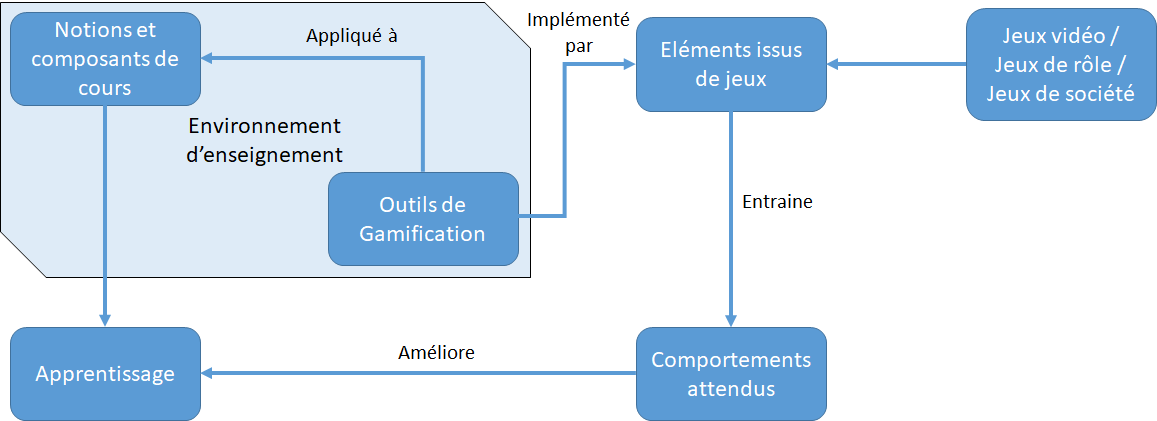
\includegraphics[width=\linewidth]{Images/Framework_Gamification_Education.png}
    \caption{Framework d'application, fonctionnement et résultats de la gamification à un contexte d'enseignement}
    \label{fig:framework_gamif}
\end{figure}

\subsubsection{Montée de niveau et gain d'expérience}
Outil classique et très fréquemment utilisé, la montée de niveau est simple à comprendre et expliquer aux participants : le niveau du joueur augmente d'un cran dès qu'un certain nombre de point d'expérience est acquis. On peut définir dans le cadre du jeu que le nombre de points requis est constant pour chaque montée de niveau, ou à l'inverse que chaque niveau atteint demande plus de points que le précédent. La deuxième option permet de rendre chaque montée plus gratifiante que les précédentes, tant que l'augmentation du nombre de points requis n'est pas disproportionnée ; si la montée de niveau devient trop laborieuse, on court le risque de démotiver les participants qui se contenteraient alors du niveau atteint jusqu'alors. De même, si augmentation il y a, elle doit suivre une logique et une formule déterminée afin que les montées de niveaux ne semble pas impossible sans une implication excessive dans le jeu. \par

Mettre en place un système de niveau dans un enseignement peut se faire de différentes manières. On peut par exemple définir que chaque participation en cours, que ce soit en répondant oralement ou en allant résoudre un exercice au tableau, fait gagner à l'étudiant un certain nombre de points. Les exercices à faire à la maison ou à rendre en fin de séance ainsi que les examens en rapporteraient également. A chaque niveau gagné, on pourrait remettre une petite récompense à l'élève, liée ou non au cours, physique ou virtuelle. La récompense n'aurait pas besoin d'être conséquente mais sa simple existence permettrait de donner un but à cette montée. Une seconde manière de faire serait simplement que chaque grande notion de cours comprise et validée par une évaluation fasse monter l'étudiant d'un niveau directement. Le niveau devient alors une mesure de la compréhension globale de l'enseignement, bien que cela puisse décourager ceux qui auraient quelques niveaux de retard sur le reste de leur classe. Pour contrer cela, insister sur les notions incomprises auprès des concernés pour les ramener au même niveau que les autres, aussi bien en terme de connaissance que de jeu, semble une bonne solution. Un exercice supplémentaire à réaliser chez soi et donnant une quantité légèrement moindre de point  permettrai de compenser ce retard, de permettre à l'étudiant de s'entraîner et de ne pas sortir du jeu. 

\subsubsection{Succès et badges}
Un autre outil phare du jeu vidéo relativement simple à appliquer est le système de succès ("Achievements") et de badges. La première apparition de ce système dans le jeu vidéo date de 1982 où Activision envoyait aux joueurs leur fournissant une photo de leur meilleur score dans un de leur jeu un patch vestimentaire exclusif. Plusieurs jeux vidéos ont par la suite inclus des contenus cachés disponibles en réalisant des actions précises, comme le jeu E-Motion sorti sur Amiga en 1990, ou des titres et badges affichés sur le profil du joueur et visibles même en dehors du jeu, comme le jeu de rôle massivement multijoueur en ligne World of Warcraft. Le système de succès et de badge a réellement commencé à se démocartiser grace à la console de jeu XBox 360 de Microsoft où une majeure partie des jeux proposaient des succès plus ou moins recherchés et complets, allant de simplement terminer une partie du jeu à réaliser des actions longues et complexes durant sa partie. \par

Les succès sont une composante de gratification assez simple à appliquer durant un enseignement. On peut imaginer que chaque travail pratique réalisé, rendu et réussi, ou chaque grande notion de cours validée par une évaluation, permette l'obtention d'une badge (physique ou numérique) afin de témoigner de la réussite de l'étudiant. On peut également lier l'attribution de badges à la montée de niveau de l'élève comme précédemment évoqué, en guise de récompense pour avoir atteint un niveau prédéfini. Dans le cadre d'une récompense physique, comme un badge à imprimer, un sticker ou autre chose, l'enseignant devrait être celui qui le distribue (et si besoin le fabrique, comme dans le cas du badge). Cela permettrait un meilleur arbitrage et contrôle de leur distribution et répartition, en évitant que certains participants trichent et décide de réaliser des copies qu'ils distribueraient, diminuant la valeur de cette récompense et encourageant la triche.

\subsubsection{Classement des participants}
Majoritairement utilisé au début de l'histoire des jeux vidéos, le classement des meilleurs scores (associés ou non à un nom ou pseudonyme) est une autre forme de gratification applicable à l'enseignement. Historiquement très utilisé dans les bornes d'arcades et les premiers systèmes de jeu (notamment les micro-ordinateurs et les consoles "8 bits"), classer les participants selon leurs performances peut permettre de les motiver à mieux faire et introduire un peu de compétition et de challenge dans le cadre du cours. Il est toutefois à noter qu'un classement nominatif des étudiants pourrait décourager deux des quatre profils de joueurs, à savoir les "Explorers" et les "Socializers"~\ref{fig:bartle}. Les premiers ne cherchent pas à se comparer aux autres mais surtout à découvrir tout ce que le cours peut leur apporter ; les seconds cherchent avant tout à tisser des relations avec leurs autres joueurs et à profiter d'un esprit d'équipe. \par

Un classement général anonyme avec la possibilité d'obtenir du professeur son classement personnel par rapport au reste de la classe semble un bon compromis. On motive à la fois les "Killers" et les "Achievers" à se dépasser en leur donnant une échelle à laquelle monter et se comparer, sans afficher devant tout le groupe le niveau de chacun. On peut également imaginer que le classement personnel donné par l'enseignant ne serait pas le rang exact de l'étudiant mais par exemple dans quel quart du classement se situe l'élève. Cela fournirait également un bon outil au professeur pour savoir quel étudiant semble en difficulté ou en retard dans le jeu, lui permettant d'adapter au besoin le reste du cours.

\subsubsection{Jeu de rôle et travail d'équipe}
Comme son nom l'indique, un jeu de rôle est un genre de jeu de plateau ou de jeu vidéo où le joueur incarne un ou plusieurs personnages au sein d'un monde imaginaire plus ou moins détaillé et aux règles prédéfinies. Les plus connus et populaires inclus entre autre le jeu de rôle papier "Dungeons and Dragons" et ses déclinaisons vidéoludiques ou les séries de jeux vidéos "Pokémon" ou "The Elder Scrolls". Dans le cadre de la gamification, la mise en place d'un jeu de rôle consiste à recréer une situation réaliste où le système gamifié est mis en application. Par exemple, lors d'un cours de marketing, un élève jouera le rôle d'un vendeur et l'enseignant celui du client, afin de mettre en pratique dans un contexte fictif et ludique les notions vues en cours. Le fait d'impliquer les élèves dans l'enseignement qui leur est prodigué via un jeu de rôle montre une amélioration des résultats, d'implication et du ressenti positif des étudiants vis à vis ce celui-ci~\cite{role-playing-educ}. \par

Le travail en équipe quant à lui permet de créer un contact et une sociabilisation des participants. Afin de résoudre un but commun, ceux-ci sont dans l'obligation de coopérer, de mettre en commun leur idées et talents, et de réaliser un objectif commun où chacun est indispensable au bon fonctionnement de l'entité. En plus de satisfaire les "Socializers", il permet également aux "Explorers" de découvrir d'autres points de vue et méthodes de résolutions. En entretenant une compétition entre équipe, il est également possible de motiver davantage les "Killers" et "Achievers", permettant donc une amélioration globale de l'implication des participants. Sauf cas où certains participants sont plutôt individualistes ou travaillent mieux seuls, les travaux de groupe sont une bonne solution pour garder l'ensemble du public cible impliqué dans le jeu, et par conséquent le système gamifié. \par

Pour gamifier un cours de d'informatique, il serait possible de concevoir des exercices de mise en situation précis et concrets, où des équipes serait chacune mise face à un problème concret à résoudre, où l'enseignant pourrait jouer le rôle d'un client ou simplement de maître du jeu. Chaque membre de l'équipe détiendrait des informations différentes concernant le problème à résoudre, forçant la mise en commun et la communication au sein de l'équipe afin de comprendre et mettre en relation ces données. Chaque équipe aurait pour but de résoudre le plus vite possible de manière correcte son problème avant de rendre sa solution à l'enseignant qui se chargera de l'évaluer. Pour augmenter le défi il serait possible de limiter dans le temps la résolution de l'exercice, pour forcer la communication à être la plus efficace et claire possible. A la fin du temps imparti, chaque équipe changerait de sujet à résoudre, de composition ou les deux, pour voir si une autre configuration ou un autre objectif fonctionne mieux avec eux, et pour mettre en pratique un autre aspect de l'enseignement. Enfin, la réalisation d'un classement des équipes avec un badge exclusif ou un gain d'expérience plus important pour ses membres en fin d'exercice permettrait de mettre en pratique toutes les mécaniques précédemment abordées.

\subsection{Évaluer la réussite des étudiants}
L'évaluation actuelle des étudiants est réalisée tout au long du module par des exercices et en fin de module par un contrôle terminal. Les exercices corrigés pendant les séances avec l'enseignant et les résultats de chacun sont échangés, expliqués ou débattus. Une ou deux évaluations notées de mi-parcours ont lieu, complétées par l'évaluation finale de fin de module. \par 

Désormais, ce modèle sera complété par une évaluation par l'enseignant des notions au fur et à mesure du cours. En fonction des résultats aux exercices proposés dans le cadre du module, l'enseignant déterminera si les étudiants ont validé celles-ci ou non et pourra proposer des exercices complémentaires à effectuer pour s'améliorer à ceux qui auraient échoués. Les notions ne sont pas évaluées directement par un exercice précis, mais plutôt par croisement des différents résultats des étudiants. Les activités proposées en cours (voir~\nameref{appendix-activity-or}) sont constituées de plusieurs exercices, et sont pensées pour être aussi bien réalisées en auto-évaluation chez soi que dans le cadre des travaux dirigés. \par

\subsubsection{Activités et exercices}
La première activité prévue a pour but d'apprendre l'identification des problématiques de Recherche Opérationnelle. Les étudiants devront, pour une série de photographies présentant un cas d'application, identifier un maximum de problématiques à résoudre afin de veiller au bon fonctionnement du système. Par exemple, à quels problèmes de logistiques est confronté un aéroport ou le réseau ferré français. L'exercice consiste à donner au moins dix problématiques par cas sous forme de mots-clés ("bagages", "passagers", "parking", etc.). Dans le cas de l'auto-évaluation, une liste de mots-clés possibles sera fournie à l'étudiant une fois son exercice réalisé afin qu'il compare ses résultats. Dans le cas d'une réalisation classique en cours, l'enseignant discute les résultats qu'il avait sélectionné et ceux trouvés par les étudiants. On considérera que l'activité est réussie et validée si, pour chaque cas, au moins 80\% des réponses étaient dans la liste de l'enseignant, puis si 80\% des cas ont rempli cette condition. \par

La seconde activité valide la compréhension des graphes et de leurs propriétés et représentation. Les exercices consistent ici à déterminer de manière graphique si un graphe répond à tel ou tel critère ou certaines de ses propriétés (s'il est orienté ou non, ou son nombre de sommets par exemple), de donner leur représentation graphique ou encore de généraliser un résultat. L'évaluation est ici plus traditionnelle, chaque réponse est juste ou erronée et correspond à une question. Afin de considérer l'activité comme réussi et validée, au moins 80\% de bonnes réponses sont attendues, et aucun exercice ne doit avoir été ignoré complètement. On attend de l'étudiant qu'à défaut d'avoir la bonne réponse, il puisse au moins fournir un raisonnement et une ébauche de solution. \par

Les deux activités suivantes sont complémentaires et visent à résoudre des problèmes par des graphes et à effectuer diverses démonstrations. Ces exercices demandent de réaliser des graphes répondant aux énoncés, de montrer des propriétés des graphes et d'en déduire des résultats ou encore d'appliquer des algorithmes  à des graphes donnés. Leur validation demande 80\% de bonnes réponses et que les exercices soient au moins en parti réalisés, de la même manière que la seconde activité. \par

Une activité d'entraînement réalisable à distance sera proposable afin que les étudiants puissent réviser leurs notions tout en réalisant un jeu. L'exercice n'aura pas de limite de temps ou de nombre de réalisations. Les étudiants seront soumis à des questions ou à des affirmations accompagnées ou non d'un graphe ou d'une représentation graphique. Pour chacune d'elles, plusieurs choix de réponses seront disponibles, sous la forme d'une réponse par vrai ou faux, de plusieurs réponses mutuellement exclusives ou de réponses à choix multiples admettant plusieurs réponses. Le but de l'exercice est de vaincre un "boss de fin de niveau" possédant un nombre de point de vie, chaque bonne réponse lui faisant perdre un montant défini à l'avance. En revanche, l'étudiant possède lui aussi un nombre de point de vie et chaque mauvaise réponse lui faisant perdre un montant également. Le but de l'exercice est de vaincre le "boss" sans perdre tous ses propres points. Un classement personnel sera ensuite montré à l'étudiant avec ses meilleurs résultats, c'est à dire son nombre de bonnes réponses et son nombre de points de vie restant à la fin de l'exercice. Un classement global de sa promotion pourrait également lui être proposé. Afin d'encourager davantage à continuer à jouer, les mauvaises réponses afficheront une explication de la réponse attendue. \par

Une dernière activité, réalisable par groupes de trois ou quatre étudiants, est également envisageable et proposerait un entraînement sur des exercices plus poussés. Trois sujets d'exercice sont proposés successivement à chaque groupe : réalisation de graphes, démonstrations de propriétés et analyse de graphes. Ces sujets sont complémentaires aux activités précédentes en poussant leur difficulté plus loin afin que le travail de groupe soit nécessaire à leur réalisation. Chaque résolution de sujet est chronométrée, puis chaque groupe rend sa copie et passe au sujet suivant, avant de répéter le processus une dernière fois. Une fois les trois copies par groupe rendues, les exercices sont corrigés puis notés par l'enseignant en présence des élèves. Les groupes seront ensuite classés selon leurs résultats. La bonne communication au sein du groupe et la participation de chacun seront les éléments clés de la réalisation de l'activité.

\subsubsection{Modalités d'évaluation}
Le taux de bonnes réponses de 80\% a été choisi afin de s'assurer une compréhension globale des notions du cours et encourager les étudiants à les réviser et les approfondir pour les repasser en auto-évaluation par la suite si le taux n'est pas atteint. Il est tout à fait possible de moduler ce taux en y appliquant une variable $x$ d'une valeur comprise dans l'intervalle $[0,8\;;1,2]$. Cette variable permet de moduler le taux de 64\% à 96\% et ainsi d'adapter l'évaluation aux résultats des étudiants. \par

En cas d'exercice ou d'activité réalisée en groupes, par exemple l'identification de problématiques ou la compréhension de graphes et de leurs propriétés, la notation ne change pas mais la consigne peut varier légèrement. Pour encourager l'échange entre les étudiants et la confrontation de pistes et d'idées diverses, la difficulté de l'exercice devrait être supérieure pour demander une réflexion plus complète. Ce type de travaux ne rentre pas complètement dans l'évaluation des acquis mais davantage dans la stimulation de la réflexion et la compréhension plus profonde des notions abordées par le cours. L'incorporation d'une composante de jeu de rôle peut renforcer le travail par groupe en mettant en situation les étudiants et en leur demandant l'adoption d'un point de vue de réflexion différent. 

\subsection{Gamification des activités et organisation}
La gamification du cours de Recherche Opérationnelle se fera selon deux axes principaux : un système de gain d'expérience et de montée de niveau, et un système de badges pour récompenser les étudiants. \par

Les étudiants commenceront le module avec un niveau d'expérience de 1 et gagneront un niveau tous les 250 points d'expérience acquis. Lors de la réalisation d'une activité, chaque exercice validé rapportera 50 points, qu'ils aient été effectué durant la séance de travaux dirigé ou en auto évaluation. Si l'activité est validée à 100\%, c'est à dire si chaque exercice de l'activité est réussi à $x$ x 80\%, un bonus de 100 points est attribué à l'étudiant. Un étudiant absent sans justification lors de la séance mais réalisant en auto-évaluation une activité par la suite marquera la moitié des points qu'elle devrait lui rapporter, mais aura tout de même accès au bonus. \par

Ces valeurs ont été choisies pour que l'élève monte de niveau approximativement à chaque activité, dans le but de le motiver à réaliser au mieux les exercices. Il est bien sûr possible d'appliquer à ces gains une variable $y$ comprise dans l'intervalle $[0,5\;;1,5]$ en fonction du taux de bonnes réponses demandées. Par exemple, pour une valeur de $x$ basse, on pourra baisser en conséquence $y$ pour signifier que l'exercice était simple, et inversement avec une valeur de $x$ plus élevée. \par

L'attribution de badges pourra se faire aussi bien pour récompenser une montée de niveau ou une réussite dans le cadre de l'enseignement. Ces badges peuvent aussi bien être virtuels et accessible via un service à déterminer, il est possible de les imprimer et de les distribuer. Si récompenser chaque montée de niveau risque de de diminuer l'impact positif de la récompense, une attribution à chaque niveau pair atteint permet une récompense rapide (le niveau de départ étant fixé à un), puis semi-régulière par la suite afin de toujours récompenser les efforts. Un badge peut être donné également quand une activité est validée à 100\%, voire quand tous les exercices de l'activité sont eux même validés et justes à 100\%. Dans le cas d'un exercice par groupe, un badge peut être attribué à l'équipe ayant réalisée le meilleur score ou ayant réalisé l'exercice le plus rapidement avec le moins d'erreurs, motivant à la fois le travail de chacun et la collaboration des membres. \par

Il serait également possible de réaliser un classement par niveau des étudiants afin que chacun puisse voir où il se situe par rapport à sa promotion. Cependant,  afin d'éviter le développement d'une compétition, la démotivation ou le surmenage~\cite{gamif-educ}, il serait judicieux de proposer un classement sur la base du volontariat s'il n'est pas anonyme. Ainsi, les plus compétitifs pourraient se comparer et chercher à faire mieux que les autres, tandis que les autres pourraient profiter des autres aspects de la gamification sans pression. Le niveau final atteint de chaque étudiant, une fois comparé par l'enseignant au reste de la promotion, pourrais également constituer une forme de note de contrôle continu ; un niveau élevé reflète une bonne compréhension et application des notions vues en cours.

\subsection{Exercices de Recherche Opérationelle gamifiés}
\begin{table}
    \begin{center}
        \begin{tabular}{|p{0.33\linewidth}|p{0.33\linewidth}|p{0.33\linewidth}|}
        \hline
        \textbf{Types d'exercice rencontrés dans le cours  de Recherche Opérationnelle} & \textbf{Activité gamifiée} & \textbf{Fonctionnement} \\ \hline
         Définitions et leur application &  Application Anki &  Entraînement auto-évalué \\ \hline
         Représentation d'un graphe &  Jeu de rapidité &  Points selon vitesse de rendu et erreurs \\ \hline
         Modélisation et résolution de problèmes &  Montée de niveau &  Déblocage de l'exercice suivant \\ \hline
         Le Duc de Densmore &  Jeu de rôle en équipe & Badge pour l'équipe la plus rapide avec la bonne réponse \\ \hline
         Détection de structures dans un graphe &  Montée de niveau &  Déblocage de l'exercice suivant \\ \hline
         Plus court chemin &  Jeu de rôle &  Résolution d'une quête avec poids minimal \\ \hline
         Application d'un algorithme &  N/A &  Résolution traditionnelle \\ \hline
         Coloration d'un graphe & Jeu de rapidité & Points selon vitesse de rendu et erreurs \\ \hline
         Couplage &  Jeu de rôle, pilotage &  Auto assemblage, pilotage d'une autre solution \\ \hline
         Modélisation de programmation linéaire &  Jeu de rapidité, jeu de rôle &  Déterminer une réponse (code) pour débloquer l'exercice suivant \\ \hline
        \end{tabular}
        \label{tab:OR_Exercices_Application}
        \caption{Exercices du cours de Recherche Opérationnelle et leur mise en place gamifiée}
    \end{center}
\end{table}

Chacune des grandes notions du cours de Recherche Opérationnelle est abordé dans un exercice qui lui est dédié. En plus des grands concepts de gamification à appliquer au cours, chacun d'entre eux peut être ciblé par un type d'élément de jeu précis et lui correspondant. Un tableau~\ref{tab:OR_Exercices_Application} les recensant nous permet de faire facilement le lien entre chaque notion/exercice et sa mise en place pratique dans l'environnement gamifié du cours. \par
Afin de réviser les définitions de cours, une implémentation de l'application Anki est possible afin de réaliser un travail en auto-évaluation. L'application Anki~\cite{anki-site} permet à chacun de réaliser un application de révision active (consistant à se rappeler des réponses à des questions données plutôt que relire celles-ci sans arrêt) en utilisant une base de données de questions/réponses personnalisée. L'application fonctionne en proposant des cartes posant une question dont la réponse est cachée, affichable via un bouton si on estime ne pas la connaître ou vouloir la vérifier. Il est possible de paramétrer la fréquence de révision et de répétition des questions posées afin de répéter celles échouées ou considérées comme plus difficiles. Grâce au support \LaTeX\ intégré, il est possible d'inclure des graphes dans les énoncés des questions, et ainsi avoir une représentation visuelle d'un cas concret. Cette application permettrait ainsi de réviser les notions de base du cours simplement et de manière personnalisée selon les besoin de chaque étudiant qui l'implémenterait. Afin de varier et chercher à stimuler la rapidité des réponses, l'add-on Speed Focus~\cite{anki-addon} permet lui de mettre en place des chronomètres pour limiter dans le temps la fenêtre de réponse et de définir l'échec ou la réussite de la carte en cours selon la volonté de les revoir dans le futur ou non. \par
Deux exercices peuvent inclure directement un système de montée de niveau, à savoir la représentation de graphes et la détection de structures. L'objectif pour les étudiants est de résoudre correctement l'exercice pour gagner un niveau, et débloquer l'exercice suivant. A la fin du cours, un classement des étudiants peut être réalisé en fonction du nombre d'exercices réalisés durant la séance. Dans le cas où un étudiant ne réussi pas à résoudre un exercice, il sera mis dans un groupe d'autres étudiants dans le même cas que lui, sur le même exercice, afin de le résoudre à plusieurs et mettre en commun leurs connaissances et stratégies. \par
L'exercice du Duc de Densmore consiste à retrouver l'assassin du dit Duc parmi une liste de suspects présents sur les lieux du crimes à différentes dates. Le coupable est ainsi le seul dont la version n'est pas compatible avec l'ensemble des autres. Les étudiants sont répartis en équipes d'enquêteurs qui doivent réfléchir ensemble, réaliser les graphes correspondant à la présence de chaque suspect et trouver (en le justifiant) le coupable. L'équipe qui la première donnera à l'enseignant le nom du coupable et la bonne démarche qui a conduit à son arrestation gagnera un badge et mettra fin au jeu. Le processus de résolution est ensuite expliqué aux autres groupes pas à pas. \par
Deux jeux de rapidité, sur la représentation d'un graphe à partir de sa liste d'arêtes et la coloration de vitesse, sont mis en place avec un fonctionnement similaire. Dans les deux cas, l'objectif est à la fois de rendre les exercices le plus vite possible à l'enseignant afin d'en réaliser le maximum, et avec le nombre de d'erreurs le plus faible possible. Chaque exercice rendu fera marquer 1 point s'il est correct, avec classement final des étudiants en fin de séance. Afin d'éviter que les étudiants ne cherchent qu'à maximiser la vitesse, un exercice incorrect sera à refaire et fera perdre le point qui aurait du être engrangé même s'il est ensuite réussi. Seule la résolution correcte d'un exercice donne l'accès au suivant. Ces jeux de rapidités permettent ainsi de stimuler la rapidité de réflexion et de mettre en place une forme de compétition au sein du groupe d'apprenants. \par
L'exercice de couplage se réalisera en deux temps. Pour commencer, un groupe de $x$ garçons et $x$ filles seront chacun identifiés par un nom (Alfred, Anna, Bernard, Béatrice, etc.) et recevront une liste confidentielle de nom de personnes "compatibles". Le groupe devra ensuite déterminer, sans que quiconque dévoile sa liste, la configuration optimale de couples "compatibles" pour minimiser le nombre de "célibataire". Une fois cette partie effectuée, l'enseignant demande au reste du groupe si quelqu'un possède une meilleure solution, et la personne la plus rapide ira proposer, grâce aux listes, une meilleure configuration. En cas d'échec, on répète l'opération. \par
Le jeu de rôle appliqué à l'exercice du plus court chemin se basera sur une graphe orienté et pondéré. Les étudiants endosseront le rôle d'un aventurier devant attendre une relique en aidant sur son chemin les habitant du royaume. Cependant, ils doivent également arriver avant les autres, et devront, tout en traversant les villages (représentés par les arêtes du graphes) effectuer le travail le moins long possible (le poids des arêtes correspond au temps passé à travailler). Les étudiants arrivant en premier à la relique en aillant effectué par conséquent le travail le moins long seront décorés d'un badge. \par
La modélisation de programme linéaire combinera à la fois une jeu de rapidité et de rôle. Chaque groupe d'étudiant devra résoudre graphiquement un programme linéaire donné. Les valeurs ainsi déterminées seront à communiquer à l'enseignant, et correspondent au code débloquant l'exercice suivant. Le but de chaque équipe est ainsi à la fois de résoudre correctement ces programmes linéaires en endossant le rôle d'un agent secret, et d'en résoudre un maximum le plus vite possible. Un classement des équipes sera réalisé en fin de cours. \par
Enfin, seul point qui ne sera pas gamifié, il est ressorti que l'application d'un algorithme à un graphe donné est plus efficace lorsqu'effectué de manière plus traditionnelle. Pour ce faire, un étudiant sera choisi par l'enseignant et envoyé au tableau dessiner le graphe auquel appliquer l'algorithme, et le déroulera. Si l'étudiant n'y arrive pas, ses camardes pourront l'aider ou le rejoindre afin de tenter une autre manière de l'appliquer. Cette méthode permet aux étudiants sélectionnés, le plus souvent et si possible ceux ayant compris les notions de base mais pas les plus spécifiques, de comprendre par la pratique, et au reste du groupe de participer également à cette résolution et d'y assister.

\subsection{Rôle de l'enseignant}
La simple mise en place de ces activités seules ne permettra pas d'améliorer suffisamment l'apprentissage et l'engagement des étudiants. L'enseignant a un rôle actif à jouer dans la forme, l'évolution et la réalisation de son enseignement par ses exercices ses retours. La mise en place de "Techniques de Rétroaction en Classe" (ou TRC)~\cite{gamif-CATs}, ou "Classroom Assessment Techniques" (ou CATs) en anglais, lors des cours peut accompagner cette gamification afin de la réorienter, la faire évoluer en fonction des retours des étudiants. Les TRC permettent aux étudiants d'obtenir des informations sur leur avancement dans le cours, à quel point ils ont atteint ou non les objectifs, et d'avoir ainsi un retour en temps réel et objectif de la part de leur enseignant. Ces exercices d'une durée de cinq à vingt minutes en général donnent également à l'enseignant une bonne idée du niveau général du groupe d'apprenant concerné. \par

Les TRC sont des exercices centrés sur l'amélioration de l'apprentissage, aussi bien du coté des élèves que de l'enseignant. Ce dernier les met en œuvre sur un certain nombre de séances planifiées en amont, les adapte selon les résultats et le niveau des élèves et selon ses méthodes, et fournit aux étudiants un retour sur leurs compétences et leurs savoirs acquis. Les étudiants peuvent en retour améliorer leurs stratégies d'apprentissage en fonction de leurs résultats, en sachant que ces exercices anonymes et non notés sont un entraînement régulier. \par

Pour M. Daele~\cite{gamif-CATs}, les TRC sont basés sur sept présupposés issus de la recherche sur la pédagogie : 
\begin{itemize}
    \item "La qualité de l’apprentissage des étudiants dépend en grande partie de la qualité de l’enseignement
    \item Pour accroître leur efficacité, les enseignants devraient définir des objectifs pédagogiques puis fournir du feedback aux étudiants à propos de la façon dont ils sont en train de les atteindre
    \item Pour améliorer leur apprentissage, les étudiants ont besoin de recevoir un feedback approprié, rapide et régulier mais ils doivent aussi apprendre à évaluer eux-mêmes leur propre apprentissage
    \item Le type d’évaluation des enseignements qui permet le plus d’améliorer l’enseignement est celui qui correspond aux problèmes et aux questions que l’enseignant se pose à lui-même, ce qui veut simplement dire que le mieux est que l’enseignant puisse interagir directement avec les étudiants à ce sujet
    \item Le défi intellectuel et systématique constitue un moteur important de motivation, de développement et d’innovation chez les étudiants, et l’évaluation formative en classe peut y contribuer
    \item Les TRC ne demandent pas une formation particulière et elles peuvent être mises en place en classe par des enseignants de toutes les disciplines
    \item En collaborant avec des collègues et en impliquant activement les étudiants dans les TRC, les enseignants peuvent développer leurs compétences et leur satisfaction à enseigner"
\end{itemize}
\par 

Dans le cadre du cours de Recherche Opérationnelle, on peut imaginer qu'à partir de la deuxième séance, cinq minutes soient accordées à la fin du cours afin que les étudiants répondent à quelques questions simples sur des notions du cours précédent et à une ou deux questions sur une notion abordée le jour même. En complément, cinq à dix minutes en début de cours à partir de la séance suivant seraient utilisées afin d'analyser les résultats de la promotion et de discuter des points mal compris et de faire le point sur le niveau global des apprenants. L'enseignant pourra également fournir des conseils sur quelle notion retravailler en priorité ou des méthodes afin de mieux apprendre le contenu posant problème. Ces exercices placent l'enseignant dans un rôle de mentor vis-à-vis des élèves, qui additionné à la gamification des activités, lui permettront de mieux encadrer, encourager et guider la promotion pendant toute la durée du module.

\subsection{Hypothèse sur l'efficacité de la gamification}
Lors de l'année scolaire 2018-2019, l'enseignement de Recherche Opérationnel regroupait un total de cinquante-sept étudiants (voir \nameref{appendix-notes-or}). De ces résultats, nous pouvons en déduire divers taux qui serviront à vérifier l'efficacité de la gamification. Le taux de réussite de la promotion avant rattrapages et en incluant les absents est de 73,68\%. Quatre des étudiants de la promotion n'ont pas assisté au module ou à ses évaluations, soit un taux de 7,02\% des inscrit. En les excluant de nos observations, le taux de réussite de la promotion passe à 71,70\%. On observe une répartition des notes relativement équilibrée~\ref{tab:OR_notes_stats} avec un premier quartile à 9,7, un troisième quartile à 14,8 et un indice de dispersion de 15,6. La promotion a donc globalement validé, malgré des notes allant dans les deux extrêmes~\ref{fig:OR_notes_repart}. \par

\begin{table}
    \begin{center}
        \begin{tabular}{|c|c|c|}
        \hline
        \textbf{1er quartile} & \textbf{Médiane} & \textbf{3ème quartile} \\ \hline
        9,7                   & 11,5             & 14,8                   \\ \hline
        \end{tabular}
        \label{tab:OR_notes_stats}
        \caption{Informations statistiques sur les notes de Recherche Opérationnelle de la promotion 2018-2019 en Licence 3 à l'Université Paris-Nanterre}
    \end{center}
\end{table}

\begin{figure}
    \centering
    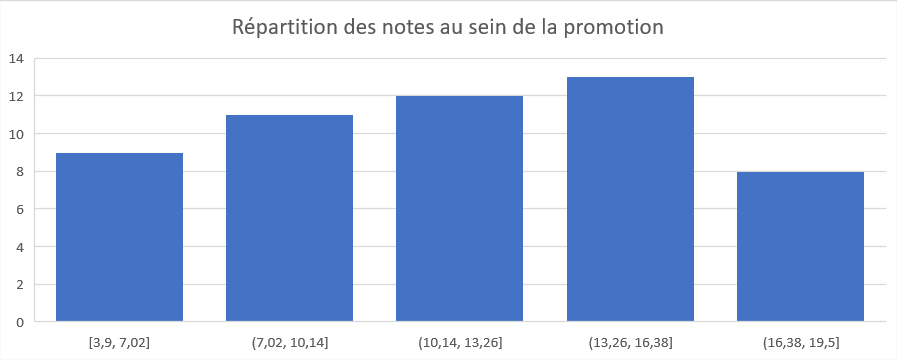
\includegraphics[width=\linewidth]{Images/Repartition_notes_RO.png}
    \caption{Répartition des notes de Recherche Opérationnelle de la promotion 2018-2019 en Licence 3 à l'Université Paris-Nanterre}
    \label{fig:OR_notes_repart}
\end{figure}


Notre hypothèse sur l'efficacité de la gamification, d'après les études réalisées~\cite{gamif-educ}, est que l'on devrait observer un taux de réussite au moins équivalent et une augmentation de la valeur des quartiles et de la note médiane. Le taux de présence devrait quand à lui baisser légèrement, tout comme l'indice de dispersion qui devrait diminuer.

\subsection{Évaluer l'efficacité de la gamification}
Afin de vérifier au mieux notre hypothèse, il nous faut pouvoir comparer les résultats attendus et obtenus à la fois du cours sans gamification et avec. Pour considérer que sa mise en application a amélioré la réussite des étudiants, la réussite globale du groupe doit avoir augmenté, mais l'écart entre les meilleurs résultats et les moins bons ne doit pas avoir augmenté pour autant. Dans le cas où cet écart se creuserait, la réussite de la gamification ne saurait être validée ; si les meilleurs le deviennent encore plus mais que les élèves en difficulté ne s'améliorent pas, la méthode n'est pas la bonne et n'a servi qu'à accentuer les différences entre les étudiants. \par

Les participants à l'expérience seront répartis dans un groupe témoin et un groupe de test. L'échantillonnage sera limité par la taille des promotions et risque de ne pas être significatif. En partant du postulat que chaque promotion fait une trentaine d'étudiants (en incluant les élèves en MIASHS parcours MIAGE et parcours Mathématiques) et qu'il y a deux promotions chaque année (formation initiale et formation en alternance), on peut imaginer deux moyens de comparer les résultats. \par

En incluant les deux promotions d'étudiants dans l'expérience, on obtient un échantillon de taille $n = 60$ environ, variant légèrement selon le nombre d'étudiants de chaque parcours\footnote{$n$ pourra être plus petit certaines années, selon le nombre d'étudiants dans les promotions, les abandons et les absents. On considérera ici $n$ comme étant à sa valeur prévue et optimale.}. Cet échantillon, bien que réduit, permet d'être relativement significatif tout de même. Il permet de comparer deux environnements et profils d'étudiants différents et d'adapter nos variables $x$ et $y$ précédemment évoquées de manière plus précise tout au loin de l'enseignement aux deux groupes. On peut ensuite réaliser l'expérience de deux manières. On peut pendant une année dispenser l'enseignement classique aux deux promotions qui serviront de groupe témoin global à $n = 60$ individus, puis lors de l'année suivante, mettre en place l'enseignement gamifié sur le groupe test, composé de la même manière de $n$ individus. On peut également lors d'une première année dispenser à une des promotions l'enseignement traditionnel et à l'autre l'enseignement gamifié, formant ainsi un groupe témoin et un groupe de test de $n = 30$ individus chacun, puis répéter le même procédé en inversant quel groupe reçoit quel enseignement une deuxième année. La deuxième méthode permet de prendre en compte l'éventuelle différence de niveau et/ou de comportement d'une promotion annuelle à l'autre. \par
    
    \cleardoublepage
% Conclusion
    \chapter{Conclusion}
    Capter l'attention et transmettre de la meilleure manière possible des connaissances sont des problématiques anciennes et qui se poseront tant qu'il restera du savoir à communiquer à de nouvelles générations. Trouver à la fois une méthode qui convienne au plus grand nombre et soit au moins aussi efficace que les méthodes déjà en application est un défi à relever continuellement et c'est dans cette continuité que ce mémoire cherche à s'inscrire. \par

Par ces activités, ces propositions d'éléments issus de jeux et les méthodes à appliquer à l'encadrement des étudiants, la démarche de ce mémoire est d'apporter sa pierre à l'édifice dans le domaine de l'apprentissage de la Recherche Opérationnelle. L'expérience proposée ici est le résultat de l'application de méthodes existantes et éprouvées à un programme d'enseignement également en pleine réécriture afin de mieux correspondre aux étudiants de la filière MIASHS/MIAGE de l'Université Paris-Nanterre. De meilleurs résultats et une meilleure implication devraient être observés du coté des étudiants et un meilleure retour sur les méthodes utilisées et la construction du cours du coté enseignant. \par

Dans le futur, une fois cette expérience réalisée et des résultats concrets obtenus, il sera possible de vérifier la justesse de notre hypothèse, de modifier et adapter au besoin les composantes du cours afin d'affiner, améliorer et compléter l'enseignement. De même, il serait possible d'appliquer cette gamification moyennant quelques adaptations à d'autres matières enseignées lors du cursus MIASHS/MIAGE, voire dans d'autres cursus.
    
    \cleardoublepage
%Table des matières
    \tableofcontents
    
    \cleardoublepage
% Bibliography
    \phantomsection
    \addcontentsline{toc}{chapter}{References}%
    \bibliography{bibliography}
    
    \cleardoublepage
% Appendices
    \appendix
    \chapter{Exemple d'activité de Recherche Opérationnelle}
    \label{appendix-activity-or}
    Ci après se trouve une partie d'un exercice donné aux étudiants lors des activités réalisées en cours de Recherche Opérationnelle. Cet extrait se compose de l'énoncé de l'exercice, des graphes concernés par celui-ci puis de la zone de réponse.


\includepdf[pages=2-4]{PDFs/activite2.pdf}
    
    \chapter{Notes de la promotion 2018-2019}
    \label{appendix-notes-or}
    Ci après les notes de la promotion 2018-2019 des étudiants en licence MIASHS parcours MIAGE et parcours Mathématiques de l'Université Paris-Nanterre ayant suivi le cours de Recherche Opérationnelle. Les notes sont anonymes et classées par ordre décroissantes. Les lignes sans notes correspondent aux étudiants aux absences non-justifiées au cours et n'ayant pas été évalués.

\centerline{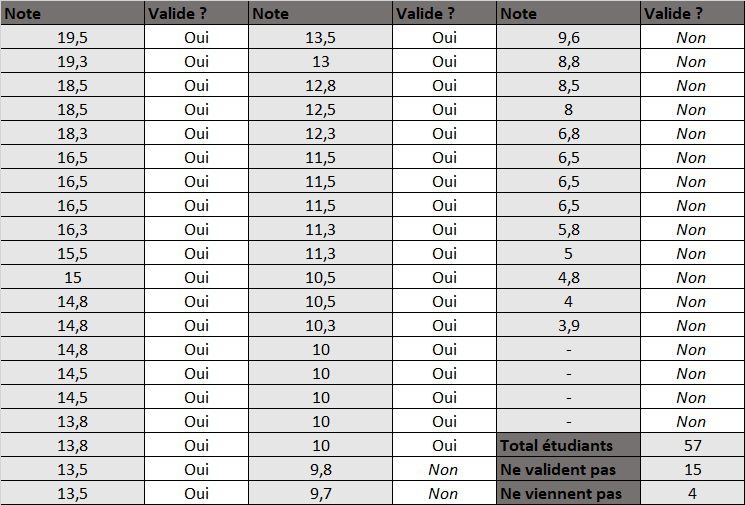
\includegraphics[width=\linewidth]{Images/Notes_RO_2018-2019.png}}


    

\end{document}
%----------------------------------------------------------------------------------------------------%
